\section{Analysis and Modeling}

\subsection{question 1: Analysis and visualization of momentum}
\subsubsection{Model Description}
To enhance the assessment of athletes’ performance, we have integrated the Analytic Hierarchy Process (AHP) with the Technique for Order Preference by Similarity to Ideal Solution (TOPSIS) for a comprehensive evaluation of the myriad factors that affect it. By combining AHP with TOPSIS, we ensure that the subjective weighting of the criteria is accounted for while preserving the precision of the evaluation methodology. This synergy between the subjective and objective aspects of the evaluation results in a more refined and accurate analysis, thereby providing a robust framework for performance assessment.\par
\textbf{Analytic Hierarchy Process (AHP)}

AHP is a compelling decision-making tool that provides a robust multi-tiered architecture that integrates and systematically considers a myriad of evaluation metrics to solve complex problems. However, an inherent drawback of AHP is that it tends to favor subjective input from decision-makers, which, despite a structured and methodical process, can distort the results due to personal bias, potentially compromising the objectivity of the decisions made. We chose AHP for the following reasons:
\begin{itemize}
    \item \textbf{Decision Framework:} AHP offers a structured model to dissect complex performance assessments into clearer, specific aspects such as technical skill and conditioning. This framework simplifies the intricate task of evaluating athletes by organizing various criteria into a clear hierarchy.

    \item \textbf{Prioritization:} AHP uses pairwise comparisons to systematically weigh and prioritize evaluation criteria and athlete performance. This process not only quantifies the importance of each criterion but also ranks athletes accordingly, providing a clear and quantitative assessment of their performance hierarchy.

     \item \textbf{Consistency Test:} AHP includes a Consistency Ratio (CR) mechanism to validate the consistency of evaluators' judgments within the decision matrix. This test ensures the dependability of the assessment, mitigating potential inconsistencies and enhancing the credibility of the results.
\end{itemize}\par
\textbf{Technique for Order Preference by Similarity to Ideal Solution (TOPSIS)}

The TOPSIS method provides a clear-cut decision-making model that prioritizes options closest to the ideal solution and furthest from the negative ideal. Key advantages of TOPSIS include:
\begin{itemize}
    \item \textbf{Data Integrity:}  TOPSIS uses raw data effectively, presenting outcomes that accurately reflect the comparative performance of alternatives.
    \item \textbf{Intuitive Logic:} With rankings based on distances to ideal and negative conditions, the method is straightforward and comprehensible.
    \item \textbf{Flexibility:}  It handles diverse data types and sample sizes without stringent limitations, offering adaptability to various decision-making situations.
\end{itemize}
\subsubsection{Data Preparation}
 In the arena of athletic performance quantification, the concept of momentum is articulated as a composite measure that is intricately woven through the amalgamation of five critical indicators, each with its designated weight to form an integrated assessment reflective of an athlete’s prevailing competitive edge. The construct of momentum is delineated along the following dimensions:
 \begin{itemize}
     \item \textbf{Situational Score:} This dimension encompasses a spectrum of sub-elements, including the number of sets secured, the cumulative game tally, the points scored in the current innings, the identity of the serving party, and the scorer of the concluding rally in the previous inning.
     \item \textbf{Lapse Situation:} Error measurement captures the instances of player missteps with a focus on the count of double faults, unforced errors, and net infractions, furnishing a portrait of error propensity during play.
     \item \textbf{Special Scoring Ability:} This category estimates the effectiveness of premium shot execution, capturing the ace rate, the frequency of winners, and the success rate of breaking an opponent’s serve, highlighting the finesse of a player’s offensive toolkit.
     \item \textbf{Fitness Score:} Calculated by the total distance covered on the court, this metric reflects the athlete’s physical stamina and vigor, which are essential for sustaining high-level performance throughout the match.
     \item \textbf{Serve Situation:} This dimension is exclusively concerned with serve-specific factors, which include the total number of serves a player has executed and the recorded speeds of those serves, offering insights into the player’s serving performance.
 \end{itemize}
\subsubsection{Modeling Process}
Firstly, for the previously screened and classified data, the judgment matrix R is constructed based on the five characteristics of the situation on the field based on the expert scoring method, and the specific values are shown in the heat map(Figure \ref{fig:JM}).
\begin{figure}[bt!]
    \centering
    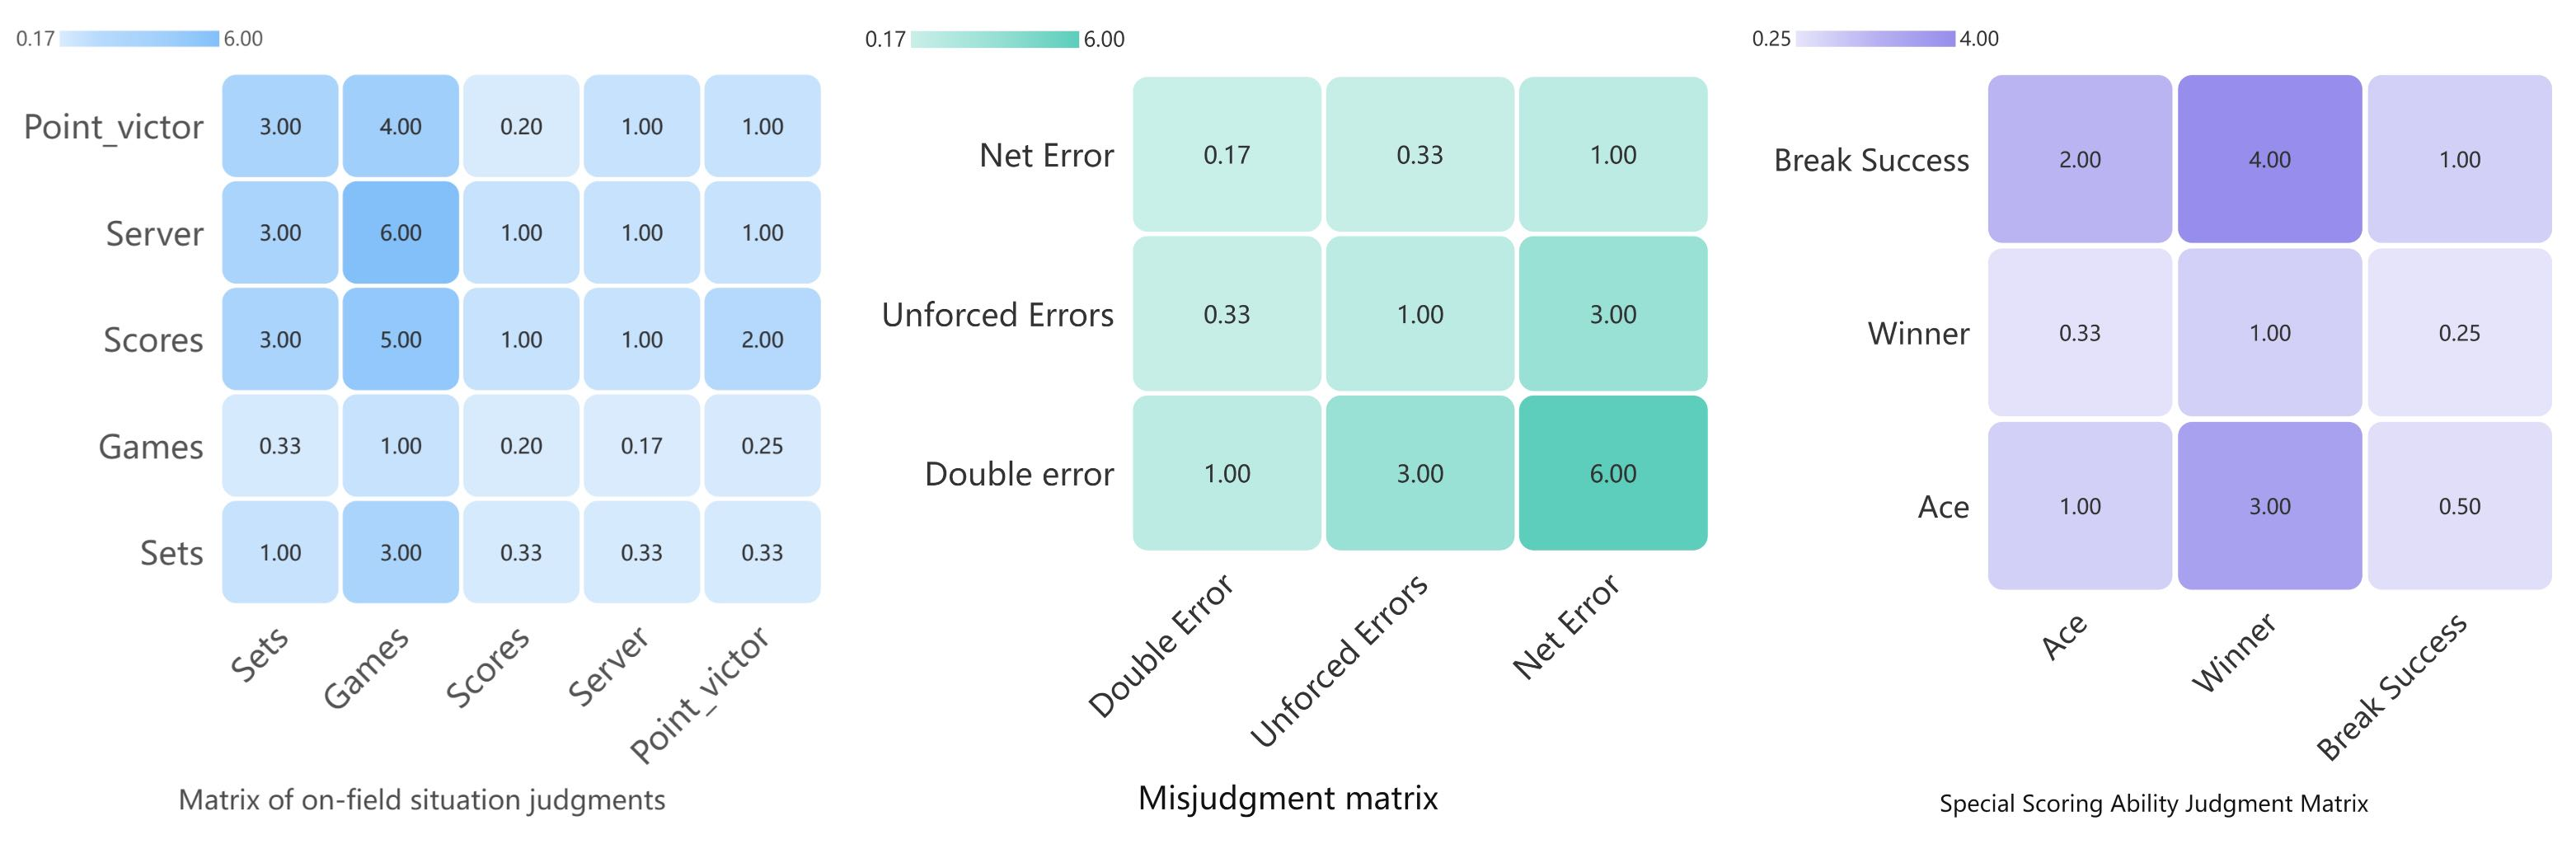
\includegraphics[width=1\linewidth]{figure/Heat Map.jpg}
    \caption{\centering Judgment Matrix}
    \label{fig:JM}
\end{figure}


The process of standardization is as follows:
\begin{itemize}
    \item Note that the maximum feature root is $\lambda_{\text{max}}$ ,then the consistency metric can be recorded as:
    \begin{equation}
        CI = \frac{\lambda_{\text{max}} - n}{n - 1}
    \end{equation}
    \item In the analytic hierarchy process(AHP), the Consistency Index (CI) is computed from the given pairwise comparison matrix. The accompanying Random Index (RI) is derived from a standard lookup table. Through the combination of CI and RI, the Consistency Ratio (CR) is determined, offering a quantifiable metric for assessing the matrix’s consistency as documented in Table \ref{tab:TCC}.
    \begin{equation}
        CR = \frac{CI}{RI}
    \end{equation}
    \begin{table}[!bt]
    \centering
    \caption{\centering Consistency Checklist} 
    \label{tab:TCC}
    \begin{tabular}{@{}lcccc@{}} % @{} removes padding at the start and end of the table
        \toprule
        & \textbf{On-court situation} & \textbf{Turnover} & \textbf{Special Scoring Ability}  \\
        \midrule
        \textbf{CI} & 0.025751807 & 0.009147232 & 0.009147339 \\
        \textbf{CR} & 0.022992685 & 0.01759083 & 0.017591037  \\
        \bottomrule
    \end{tabular}
    
\end{table}


In AHP, a concordance ratio (CR) of less than 0.1 indicates that the matrix has acceptable agreement. The data provided demonstrate that all three judgment matrices considered meet this criterion. Subsequently, the weight matrix derived by the arithmetic mean method has weights that meet the predefined criteria, which meets the requirements of our analysis. As shown in Figure \ref{fig:WPC}, the final weight proportion chart is displayed.
\begin{figure}
    \centering
    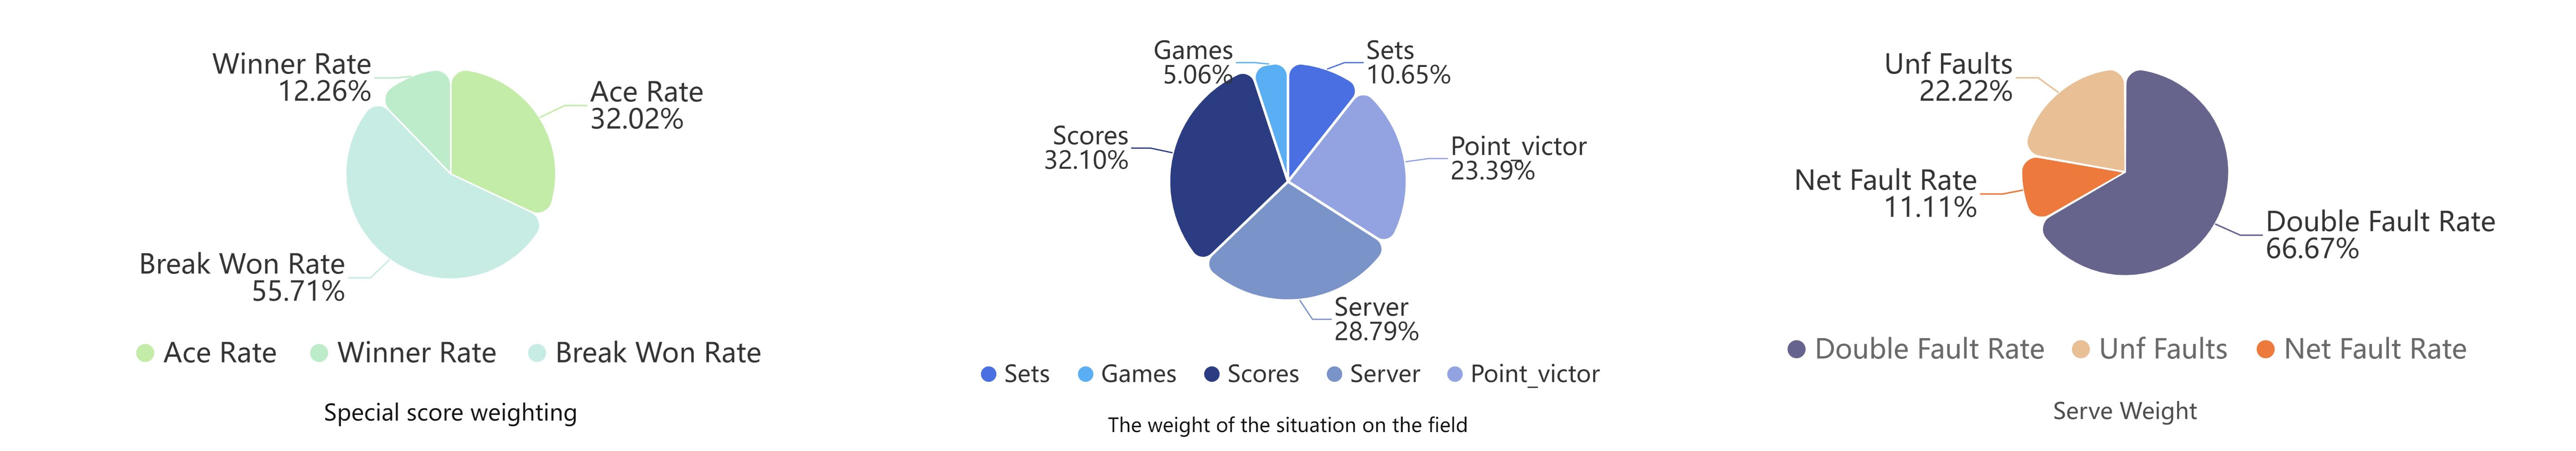
\includegraphics[width=1\linewidth]{figure/Percentage Map.jpg}
    \caption{\centering Weights Percentage Chart}
    \label{fig:WPC}
\end{figure}

\item In developing the Similarity Ranking First Technique with Ideal Solution (TOPSIS), the first step involves the forward transformation of the evaluation metrics. Consider metrics such as error score, double error rate, unforced error count, and net error rate; These represent performance attributes where smaller values have an intrinsic advantage to the person being evaluated, in this case, the player. These metrics are designated as “minimal” metrics in the assessment classification.
In order to address the different nature of the indicators within the TOPSIS framework and to ensure standardized comparisons, minimalist indicators require a conversion in the opposite direction of their original direction. This transformation converts a lower, more favorable value into a larger value, which is associated with enhanced performance in the normalized decision matrix. The positive transformation of these minimalist indicators is mathematically expressed as:
\begin{equation}
    \hat{x}_{i} = \max - x_{i}
\end{equation}
\item In order to eliminate the influence of different data indicator dimensions, it is also necessary to standardize the forward matrix, and the normalized matrix is Z, where 
\begin{equation}
    Z_{ij} = \frac{x_{ij}}{\sqrt{\sum_{i=1}^{n} x_{ij}^{2}}}
\end{equation}
In a situation where there are\textit{ n }schemes to be evaluated and \textit{m} indicators, the vector \(Z_{i}\) is used to express the values of the indicators for the ith scheme.At this time,$\ z_{i}=[z_{i1},z_{i2},\cdots,z_{im} ]$
The matrix composed of these \textit{n} vectors forms the normalized matrix Z :
 \begin{equation}
 Z_{ij}=
 \left[
 \begin{array}{cccc}
     z_{11}  &z_{12}  &\cdots   &z_{1m} \\
     z_{21}  &z_{22}  &\cdots   &z_{2m} \\
     \vdots   & \vdots  & \ddots & \vdots  \\
     z_{n1}  &z_{n2}  &\cdots   &z_{nm} \\
 \end{array}
 \right]        
 \end{equation}
 \item The previously calculated weight matrix was utilized to assign weights to the variable Z.
 \item The ideal optimal solution is \(Z^{+}\), and the ideal worst solution is \(Z^{-}\), and the formula for calculating the two is as follows:
\begin{equation}
    Z^{+} =[max\left \{ z_{11},z_{21},\cdots ,z_{n1} \right \} ,max\left \{ z_{12},z_{22},\cdots ,z_{n2} \right \},\cdots ,max\left \{ z_{1m},z_{2m},\cdots ,z_{nm} \right \}]
\end{equation}
\begin{equation}
Z^{-} =[min\left \{ z_{11},z_{21},\cdots ,z_{n1} \right \} ,min\left \{ z_{12},z_{22},\cdots ,z_{n2} \right \},\cdots ,min\left \{ z_{1m},z_{2m},\cdots ,z_{nm} \right \}]
\end{equation}
\item For the ith scheme \(Z_{i}\), calculate its distance from the optimal solution( \(d_{i}^{+}\) ) and the distance from the worst solution( \(d_{i}^{-}\) )
\begin{equation}
d^{+}_{i}=\sqrt{\sum_{j=1}^{m}{(z^{+}_{j}-z_{ij})^{2}} }
\ \ \ \ \ \ \ \ 
d^{-}_{i}=\sqrt{\sum_{j=1}^{m}{(z^{-}_{j}-z_{ij})^{2}} }
\end{equation}
\item Define the score of the ith scheme as \(S_{i}\), which is calculated as:
\begin{equation}
    S_{i}=\frac{d^{-}_{i}}{d^{+}_{i}+d^{-}_{i}}
\end{equation}

The \(S_{i}\) is the score (the Table3 shows some of the processed data)

\item After obtaining the five scores required to calculate the momentum, the AHP-TOPSIS model was used to evaluate the momentum scores, and the judgment matrix and weights were shown in Figure \ref{fig:M1} and Figure \ref{fig:M2}
\begin{figure}[bt!]
    \centering
    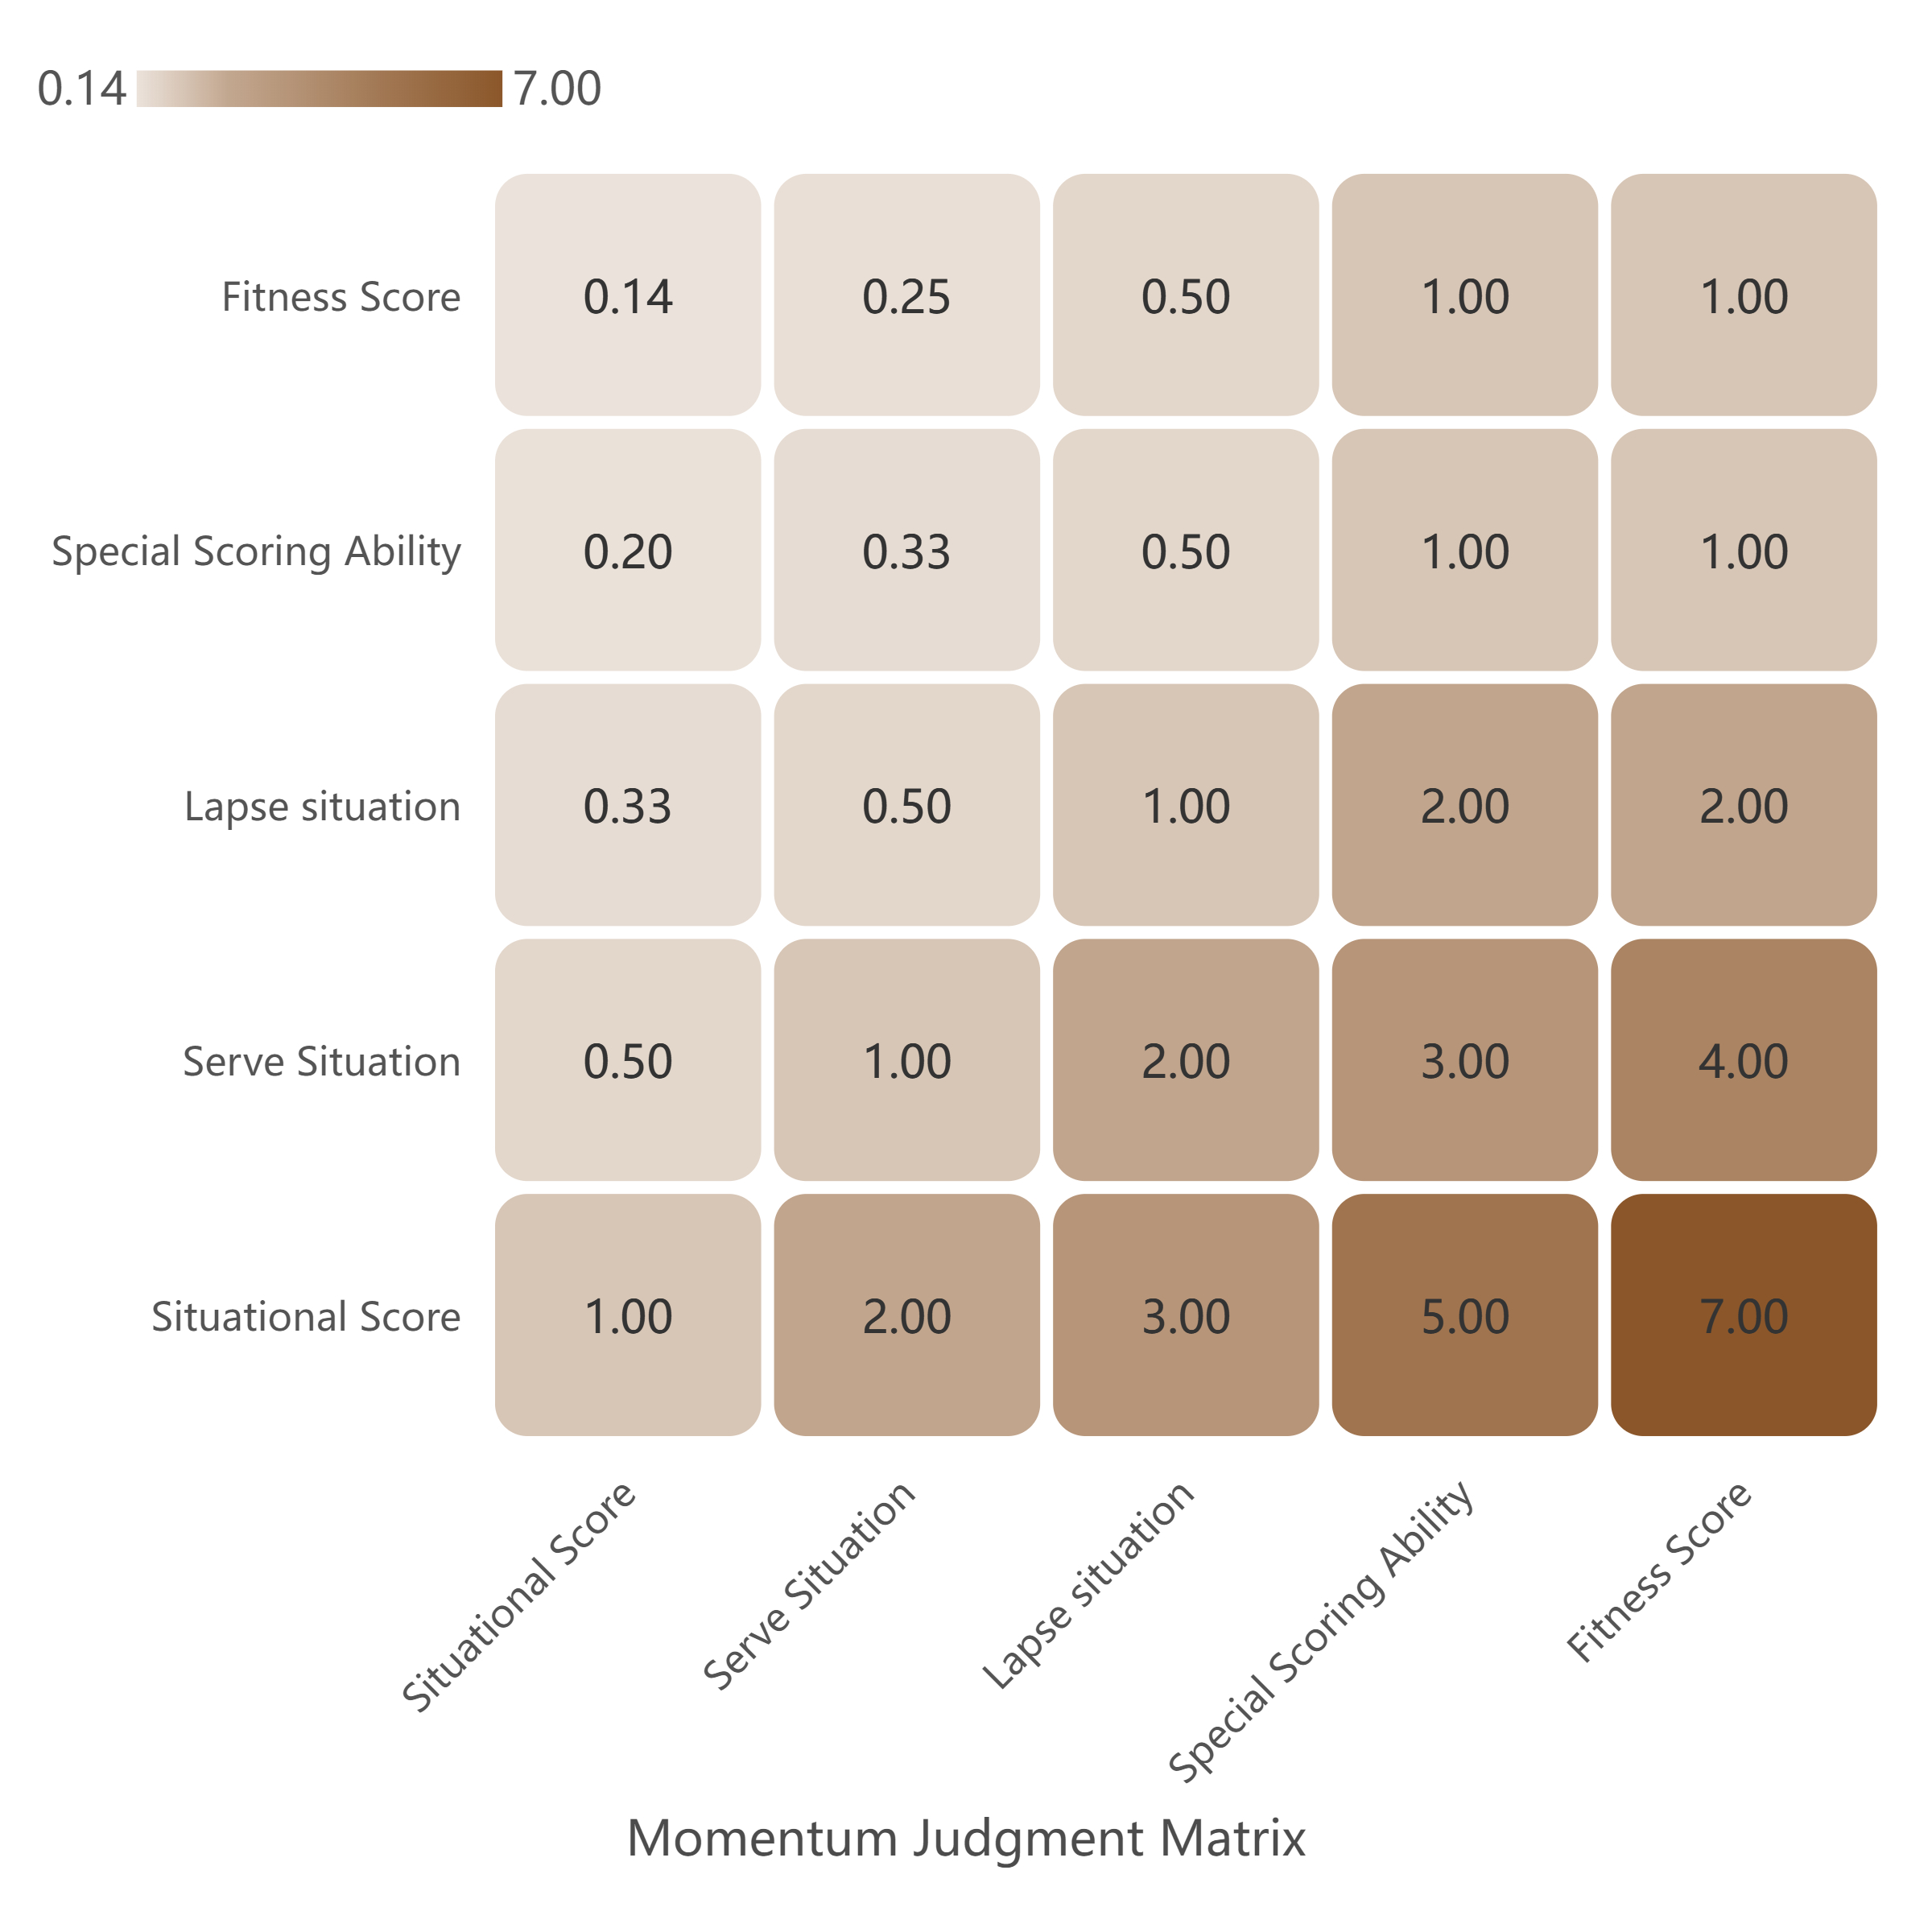
\includegraphics[width=0.5\linewidth]{figure/势头.jpg}
    \caption{\centering Momentum Judgment Matrix}
    \label{fig:M1}
\end{figure}
\begin{figure}[bt!]
    \centering
    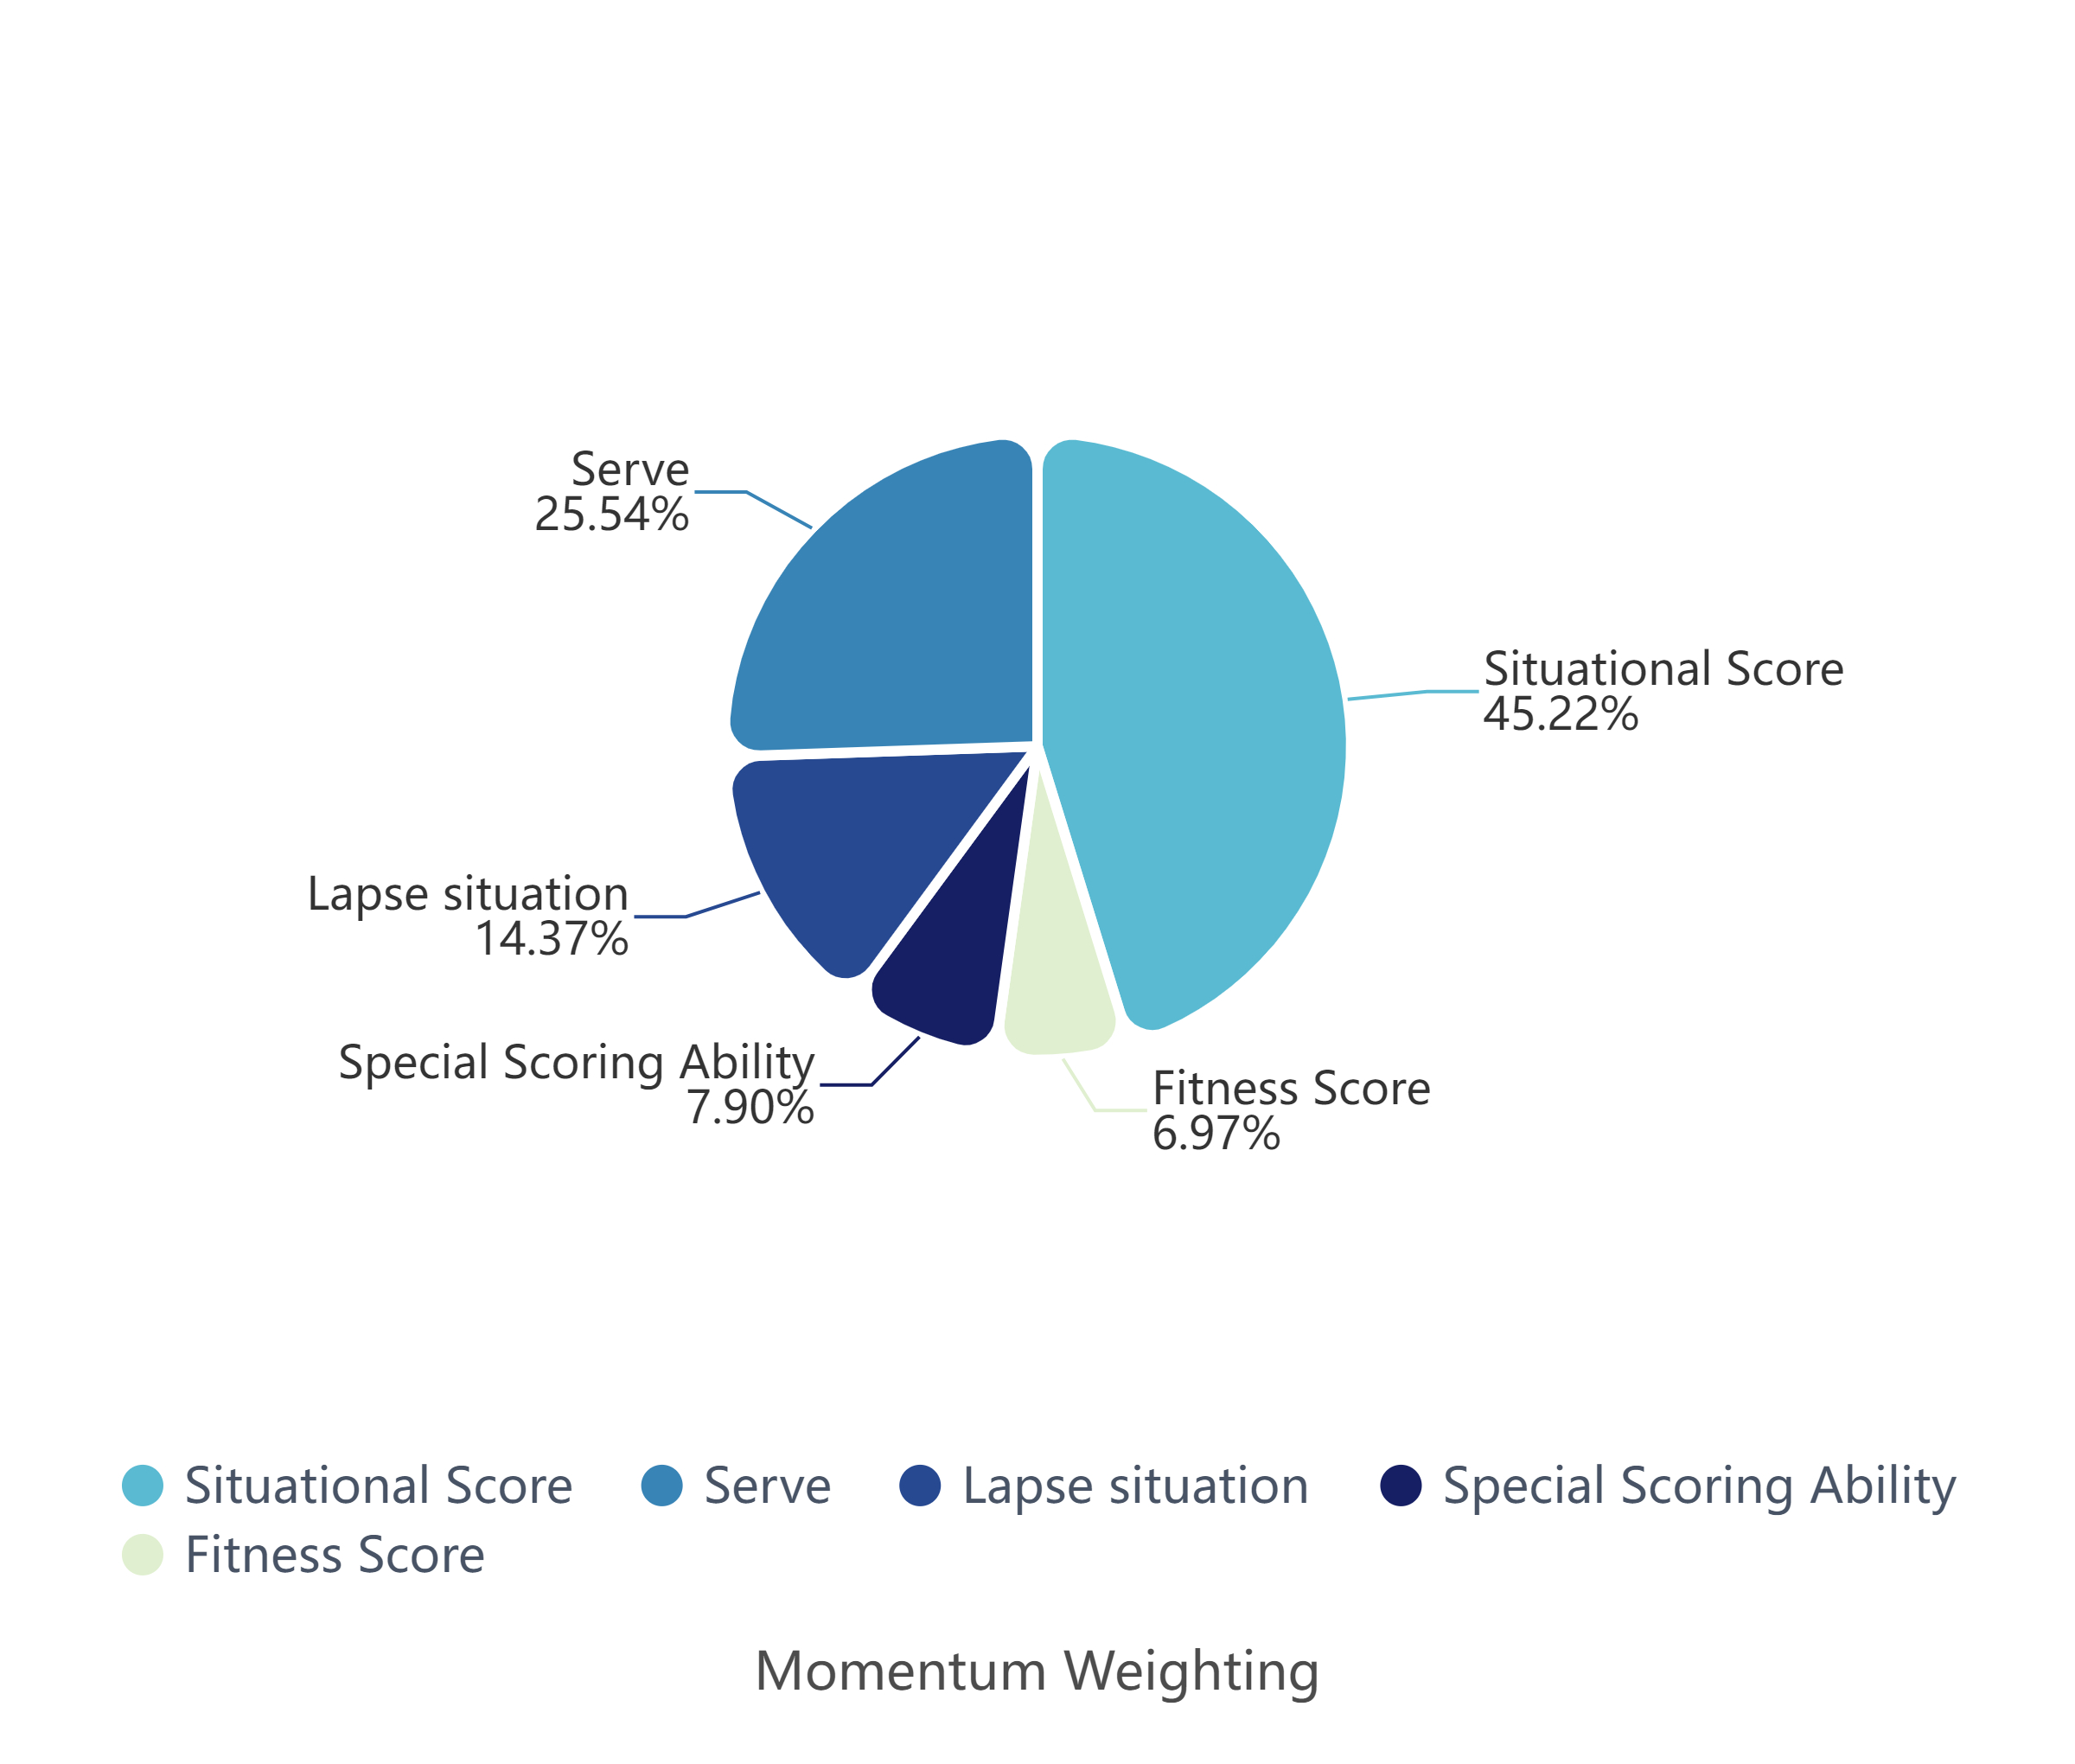
\includegraphics[width=0.75\linewidth]{figure/势头2.jpg}
    \caption{\centering Momentum Weight Chart}
    \label{fig:M2}
\end{figure}
\end{itemize}

\subsubsection{Result}
\begin{figure}[bt!]
    \centering
    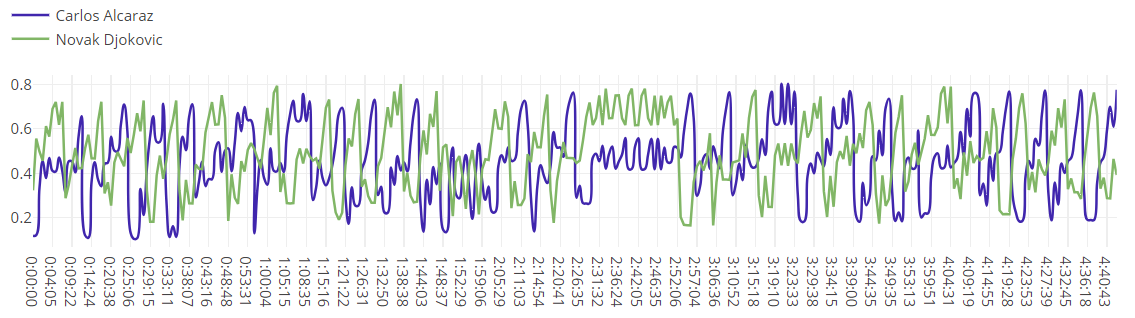
\includegraphics[width=1\linewidth]{figure/经典场.png}
    \caption{\centering Momentum Chart of the Game}
    \label{fig:M3}
\end{figure}

Figure \ref{fig:M3} shows the momentum scores of Carlos Alcaraz and Novak Djokovic in the match described in question, which is divided into five sets:
\begin{itemize}
    \item \textbf{1th:}At the beginning of the match, Novak Djokovic won the first game by overwhelmingly overpowering Carlos Alcaraz.
    \item \textbf{2th:}In the second game, the momentum of both sides was evenly scored, and it was very anxious.
    \item \textbf{3th:}In the third game, Carlos Alcaraz had a big lead, but Novak Djokovic was in the upper hand for a period of time starting at 2:31:32, which was affected by Novak Djokovic serving 32 balls as a serve (32 points in the game), and then Carlos Alcaraz regained control to win the third game.
    \item \textbf{4th:}In the fourth game, the two sides were anxious, but Novak Djokovic maintained the lead.
    \item \textbf{5th:}In the final fifth inning, Novak Djokovic had a big start but then Carlos Alcaraz rose up and scored clearly more momentum than Novak Djokovic to win the match
\end{itemize}

The visually presented line chart, or any other chart showcasing the momentum of player, highlights the hypothesis that higher momentum indicates superior performance by the player at that moment. Additionally, the disparity in momentum can serve as an indicator of the relative performance between the two players.

\subsection{question 2: Does “momentum” play any role in the match?}
\subsubsection{Brief Description of Our Solution}
In question 1, we develop a model to obtain momentum and then use it to measure players' performance. 
After evaluating the mechanism for obtaining momentum, we tend to disagree with the coach. Moreover, we developed an LSTM model to confirm our thought.

\subsubsection{Basic Data Analysis}
Perform statistical analysis on the momentum data obtained from the first question, and compare the momentum results of the athletes from both sides in each game. For the momentum comparison results, simply predict that the side with greater momentum will win, group each game by matchId, and finally calculate the prediction accuracy rate. Compare the final predicted winning rate with 50 percent, and the results after comparison are shown in Figure \ref{fig:PA}.
\begin{figure}
    \centering
    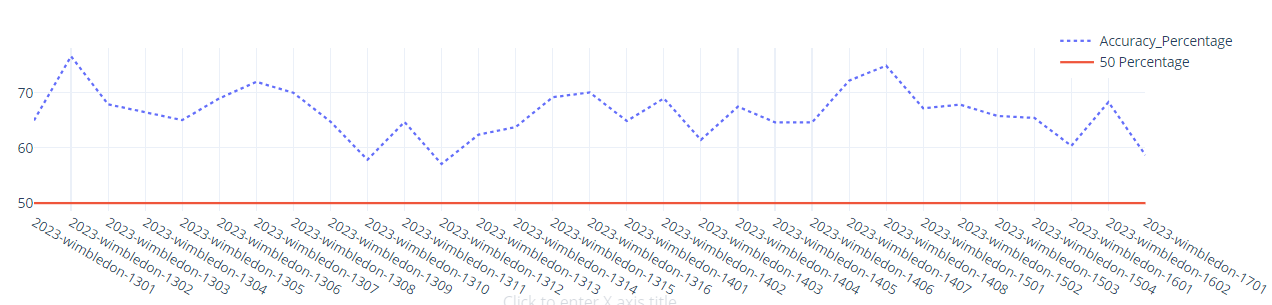
\includegraphics[width=1\linewidth]{figure/预测准确率.png}
    \caption{\centering Prediction Accuracy}
    \label{fig:PA}
\end{figure}
\subsubsection{Basic Data Analysis Results}
As can be seen from Figure \ref{fig:PA}, the accuracy rate of predicting an athlete's victory through quantified momentum exceeds 50 percent, indicating that momentum plays a role in an athlete's victory to a certain extent. Therefore, we disagree with the statement that coaching momentum is unpredictable (random).

\subsubsection{LSTM Model}
\indent LSTM (Long Short-Term Memory) is a Recurrent Neural Networks (RNN) variant designed to solve long sequence dependency problems. Recurrent neural networks can only handle close contexts but cannot get information from faraway contexts. We consider LSTM to be highly applicable to this problem for the following reasons:
\begin{itemize}
    \item \textbf{Long and Short Term Memory Mechanisms:}\ Analyzing the current tennis match should be based not only on a player's recent performance but also on the player's previous performances. The LSTM model is ideal for this problem since it consists of a " cell " memory unit, which stores and selectively forgets or passes on information to the next step. 
    \item \textbf{Advantages of RNN:}
    LSTM, a type of RNN, is often called a “black box model“due to its complex internal structure, making it challenging to understand. We can ignore the weight matrix setting process and focus solely on adjusting hyperparameters to improve the model's performance.
\end{itemize}
In this question, based on the intermediate output obtained from the AHP-TOPSIS calculation in question 1, we would like to take advantage of the above LSTM to build a model that can better predict the game's flow. Since the focus of developing the model was to confirm the correctness of our anticipated momentum, we chose to develop a base model that uses the intermediate output from momentum as input and the result of the score as output.

\subsubsection{LSTM Experiment Result}
We first initialized the model using the stochastic method and did not train it, as expected, the model had an average accuracy of 0.5. Random momentum doesn't affect the game's outcome. We aim to improve accuracy by training the model to show that predicted momentum impacts the match. \par


\begin{table}[b!]  
\caption{\centering LSTM Basic Params}% [] control the position of table
    \centering
    % \renewcommand{\arraystretch}{1.5}
    \begin{tabular}{c c}            % main part of table: {} control alignment(l,c,r)
        \toprule 
        Param & Value \\
        \midrule
        Optimizer & Adam \\
        Learning Rate & 0.001 \\
        Loss Function & BCEWithLogitsLoss \\
        Early Stop & 10 \\
        Batch Size & 32 \\
        \bottomrule
    \end{tabular}
    \vspace{10pt}
    \vspace{-5pt}
    \label{tab:lstm1}
\end{table}
Through some basic experiments, we first determined some model parameters, recorded in Table \ref{tab:lstm1}. 
Next, we experimented with several parameters whose effect on the model could not be determined. 
\begin{figure}[bt!]
    \centering
    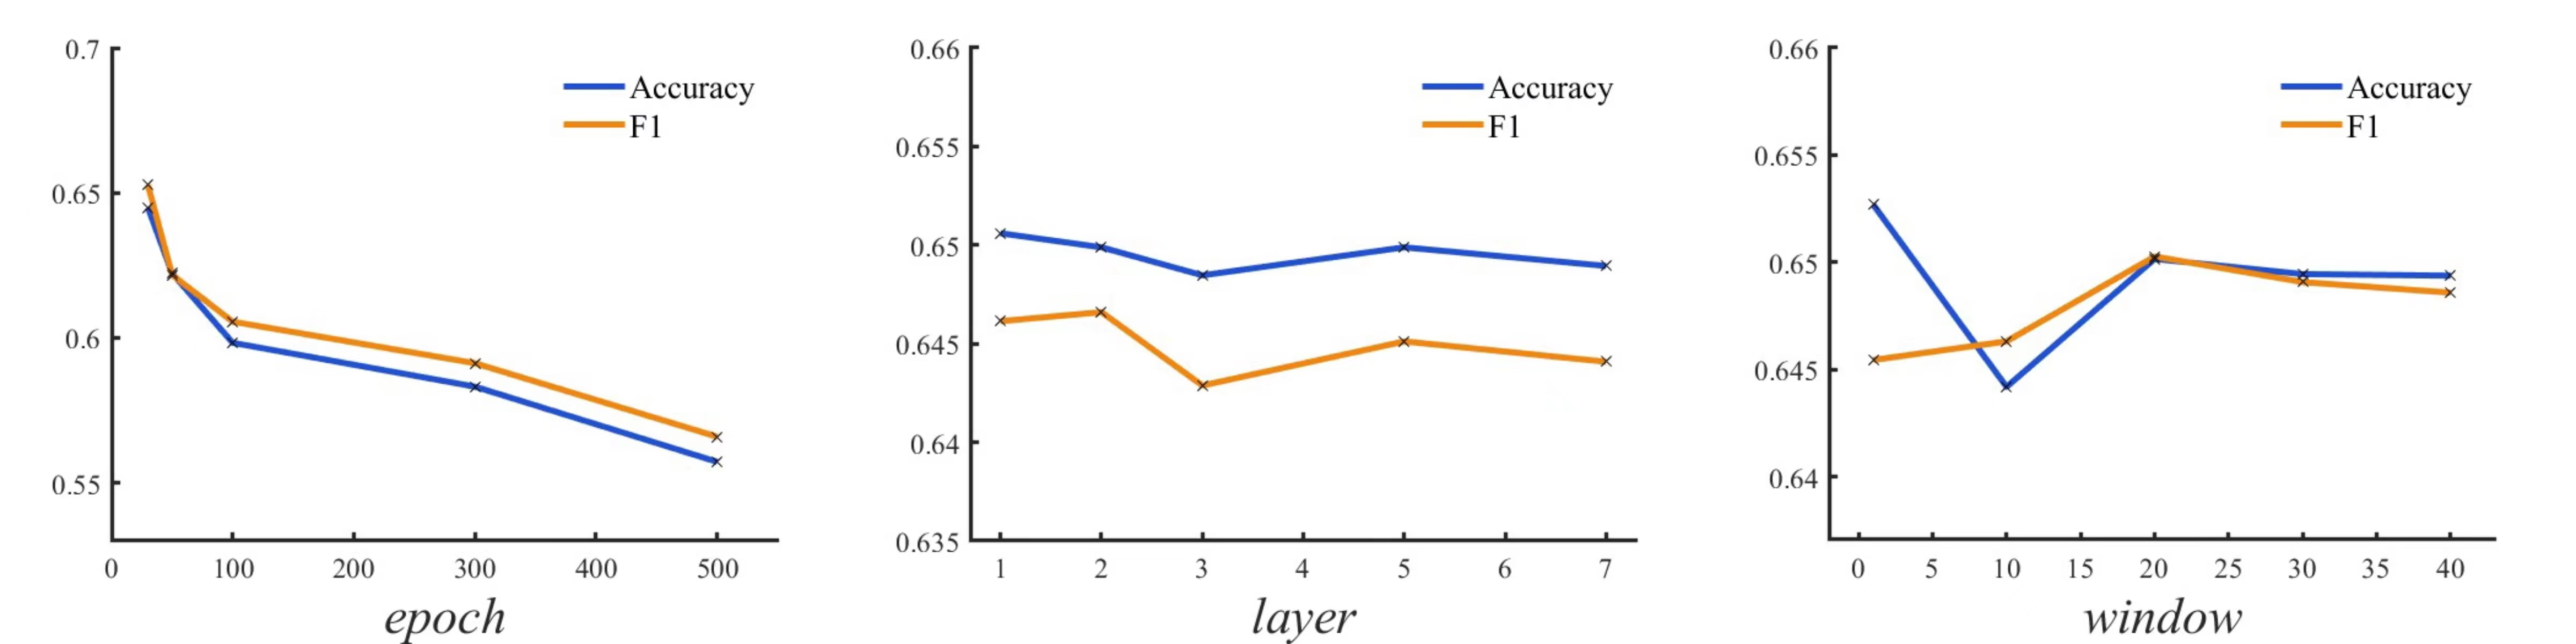
\includegraphics[width=1\linewidth]{figure/lstm1.jpg}
    \caption{\centering LSTM Parameters}
    \label{fig:lstm1}
\end{figure}
The result of our experiment is displayed in Figure \ref{fig:lstm1}. \par
During our experiments, we faced the biggest challenge in training machine models due to the lack of data and the difficulty in data augmentation. \par 
The experimental results suggest that increasing the hidden size to create a larger model by adding more parameters can lead to overfitting. Although these larger models can be trained well for multiple epochs, resulting in a low training loss, they tend to perform poorly on the test set. \par
We decided to use a small model for prediction, even though we faced difficulty achieving a satisfactory loss during the training process. However, the negligible difference between the results of the test set and the training set eventually led to a higher accuracy in the outcome.\par
In the end, we obtained an average accuracy of 0.65, which we believe is sufficient to demonstrate the correlation between momentum and game, given the varied nature of the games. \par


\subsubsection{Discussion}
\textbf{Layers of LSTM: }
After concluding our experiment, we initially attempted to explain the lack of significance of the LAYER. We considered factors such as vanishing or exploding gradients versus data complexity, but none seemed to be the right explanation. Ultimately, we determined that adding more layers increases the number of parameters. As previously discussed, this particular problem is not well-suited for large models.\par
\textbf{Window Size: }
Window Size refers to the number of scores the model will consider forward for the current situation. In the given problem, the window size plays a crucial role as it determines the memory extent that LSTM considers. According to our analysis, the model seems to struggle in making use of data from past units due to the inputs being summarized data. However, in the later developed LSTM model, we observed that the window size effect increased by inputting raw data. \par
\subsection{question 3: Find leading indicators and predict swings}

\subsubsection{Measure Swing}
As stated in the problem, what needs to be predicted is the swings of the match. So we came up with a way to quantify the swings. 
\begin{figure}[bt!]
    \centering
    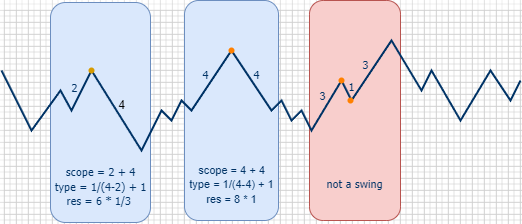
\includegraphics[width=0.75\linewidth]{figure/convert.drawio.png}
    \caption{\centering Swing Measurement}
    \label{fig:swingM}
\end{figure}
As shown in figure \ref{fig:swingM}, we use folded lines to demonstrate the game's flow. The impact of swing is divided into 2 parts:
\begin{itemize}
    \item \textbf{Scope: }Sum the lengths of the folded lines, then Find the kth power(k is used to measure the influence of the scope factor)
    \item \textbf{Type: }In figure \ref{fig:swingM}, (a) only scored 2 points in a row before experiencing a 4-game losing streak, whereas (b) was on a winning streak before the losing streak, suggests that the turning point in (b)'s situation had a greater impact. The difference in the lengths of the 2 folds should be inversely correlated with the measure, so we use the inverse proportion function.
\end{itemize}

Combining the 2 factors, the final equation is equation (\ref{equ:convert}). 
\begin{equation}
    impact = (l+r)^k \cdot \frac{1}{|l-r|+1}
    \label{equ:convert}
\end{equation}

\subsubsection{Decision Tree}
To determine the critical game indicators, we utilize the decision tree to capture various data throughout the game. \par

Decision Tree (DT) is non-parametric supervised learning that can summarize the decision rules from a series of featured and labeled data to solve classification or regression problems. \par
Meng and Huang \cite{ref1} used a decision tree model in the quantitative analysis of players' winning factors and concluded that the most important winning factor in women's tennis is the serving situation as well and the reduction of forced errors is the main way to improve the winning rate of the game. 
We took inspiration from this and used a decision tree model to predict turning points in the game while deriving the feature importance of each indicator. \par
Details about the model: 
\begin{itemize}
    \item \textbf{Gini Coefficient: }
    Using the decision tree model based on the CART algorithm for prediction, due to the use of the information entropy and the Gini coefficient of the effect is basically the same, but the calculation of the information entropy is more complex than the Gini coefficient, in addition to high-dimensional data or more noisy data, the information entropy is very easy to overfitting\cite{ref2}. Therefore, we use the Gini coefficient (gini) as a criterion parameter, the Gini coefficient (gini) index to measure the degree of stochasticity, it is defined in equation \ref{equ:dt1}
    \begin{equation}
        Gini(t) = 1- \sum_{i=0}^{c-1}{p(i|t)^2}
        \label{equ:dt1}
    \end{equation}
    \item Increase tree depth, decrease leaf nodes due to small sample size and large number of features. Higher accuracy was achieved with a maximum tree depth of 15 and 30 maximum leaf nodes.
    \item \textbf{Feature Importance: }Use Gini coefficient to determine indicator importance for the decision tree. The equation is \ref{equ:dt2}

    \begin{equation}
        I(feature)=\sum^n_{i-1}{\frac{filtered\_samples}{total\_samples}gini\_gain(decision\_node)}
        \label{equ:dt2}
    \end{equation}
    
\end{itemize}

The calculated data are normalized to obtain the characteristic importance of each indicator, which is partially plotted in figure \ref{fig:dt1}. Based on the figure, the most essential features are server, score, and point victor. These indicators have a significant impact on the game's volatility.\par


\begin{figure}[bt!]
    \centering
    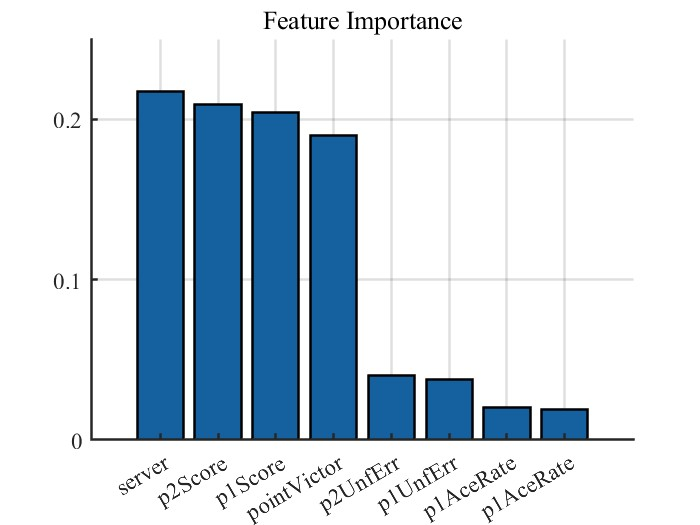
\includegraphics[width=0.6\linewidth]{figure/dt1.jpg}
    \caption{\centering Decision Tree Main Indicators}
    \label{fig:dt1}
\end{figure}

\subsubsection{Decision Tree Experiment}
\begin{table}[b!]                    % [] control the position of table
\caption{\centering Decision Tree Evaluation}
    \centering
    % \renewcommand{\arraystretch}{1.5}
    \begin{tabular}{c c c c c }            % main part of table: {} control alignment(c c c c c )
        \toprule 
        
          & \multicolumn{1}{l}{Accuracy} & \multicolumn{1}{l}{recall} & \multicolumn{1}{l}{Precision} & \multicolumn{1}{l}{F1} \\
        \midrule
    Train   & 0.77 & 0.77 & 0.75 & 0.754 \\
    Test   & 0.75 & 0.75 & 0.725 & 0.73 \\

        \bottomrule
    \end{tabular}
    \vspace{10pt}
    \vspace{-5pt}
    \label{tab:dt1}
\end{table}

\subsubsection{LSTM Specific to The Problem}
After obtaining the primary INDICATORS using the decision tree, we replace the model inputs in LSTM with the simple processed data corresponding to those INDICATORS. Upon completion of the training, we achieved an accuracy of 0.7, which is a remarkable outcome and in accordance with our initial expectations. This result verifies that we have identified the correct and efficient indicators. However, we would like to point out that Question 3 does not require us to predict the outcome of the game but rather the swing of the game.\par
After analyzing the problem, the swing was first quantified (), followed by some adjustments to the LSTM model based on the characteristics of the problem: \par 
\begin{figure}[bt!]
    \centering
    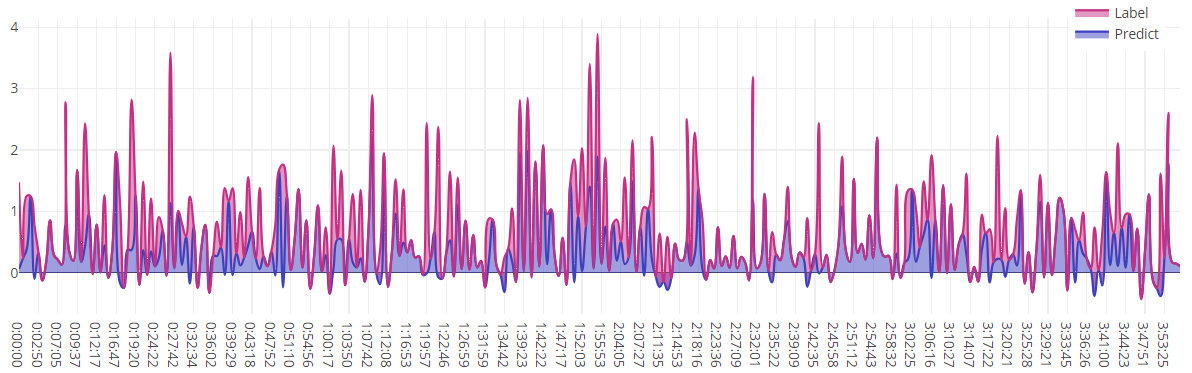
\includegraphics[width=1\linewidth]{figure/lstm2.png}
    \caption{\centering LSTM Prediction}
    \label{fig:lstm2}
\end{figure}
\begin{itemize}
    \item \textbf{Regression Model: }
    In the initial model, the problem is treated as a regression problem to predict values close to our quantized swing values. The predictions obtained by the trained model are illustrated in Figure \ref{fig:lstm2}.
    \item \textbf{Transforms Into a Categorization Problem at Output:}
    \begin{itemize}
        \item \textbf{Why?}
        We believe that for this problem, the regression problem is clearly more difficult compared to the classification problem.
        The regression model uses Mean Squared Error (MSE) as the loss function. To evaluate the effectiveness of the MSELoss, we must consider the data range. And MSELoss is less intuitive than accuracy.
        \item \textbf{How?}
        During training, we still train the model as a regression model to take advantage of the benefits offered by quantized turning points but transform the model output into a classification. Details: Set the value that is not a turning point to 0 and make the turning point value converge to 1 using the equation (\ref{equ:lstm2}). In the output, we transform the model prediction into 0/1. If it is a test, you need to do the label accordingly.
        \begin{equation}
            swing\_label =\begin{cases} sigmoid(swing)\quad ,swing>0 \\0\quad,swing=0 \end{cases}  
            \label{equ:lstm2}
        \end{equation}
    \end{itemize}
    
\end{itemize}
\begin{figure}[bt!]
    \centering
    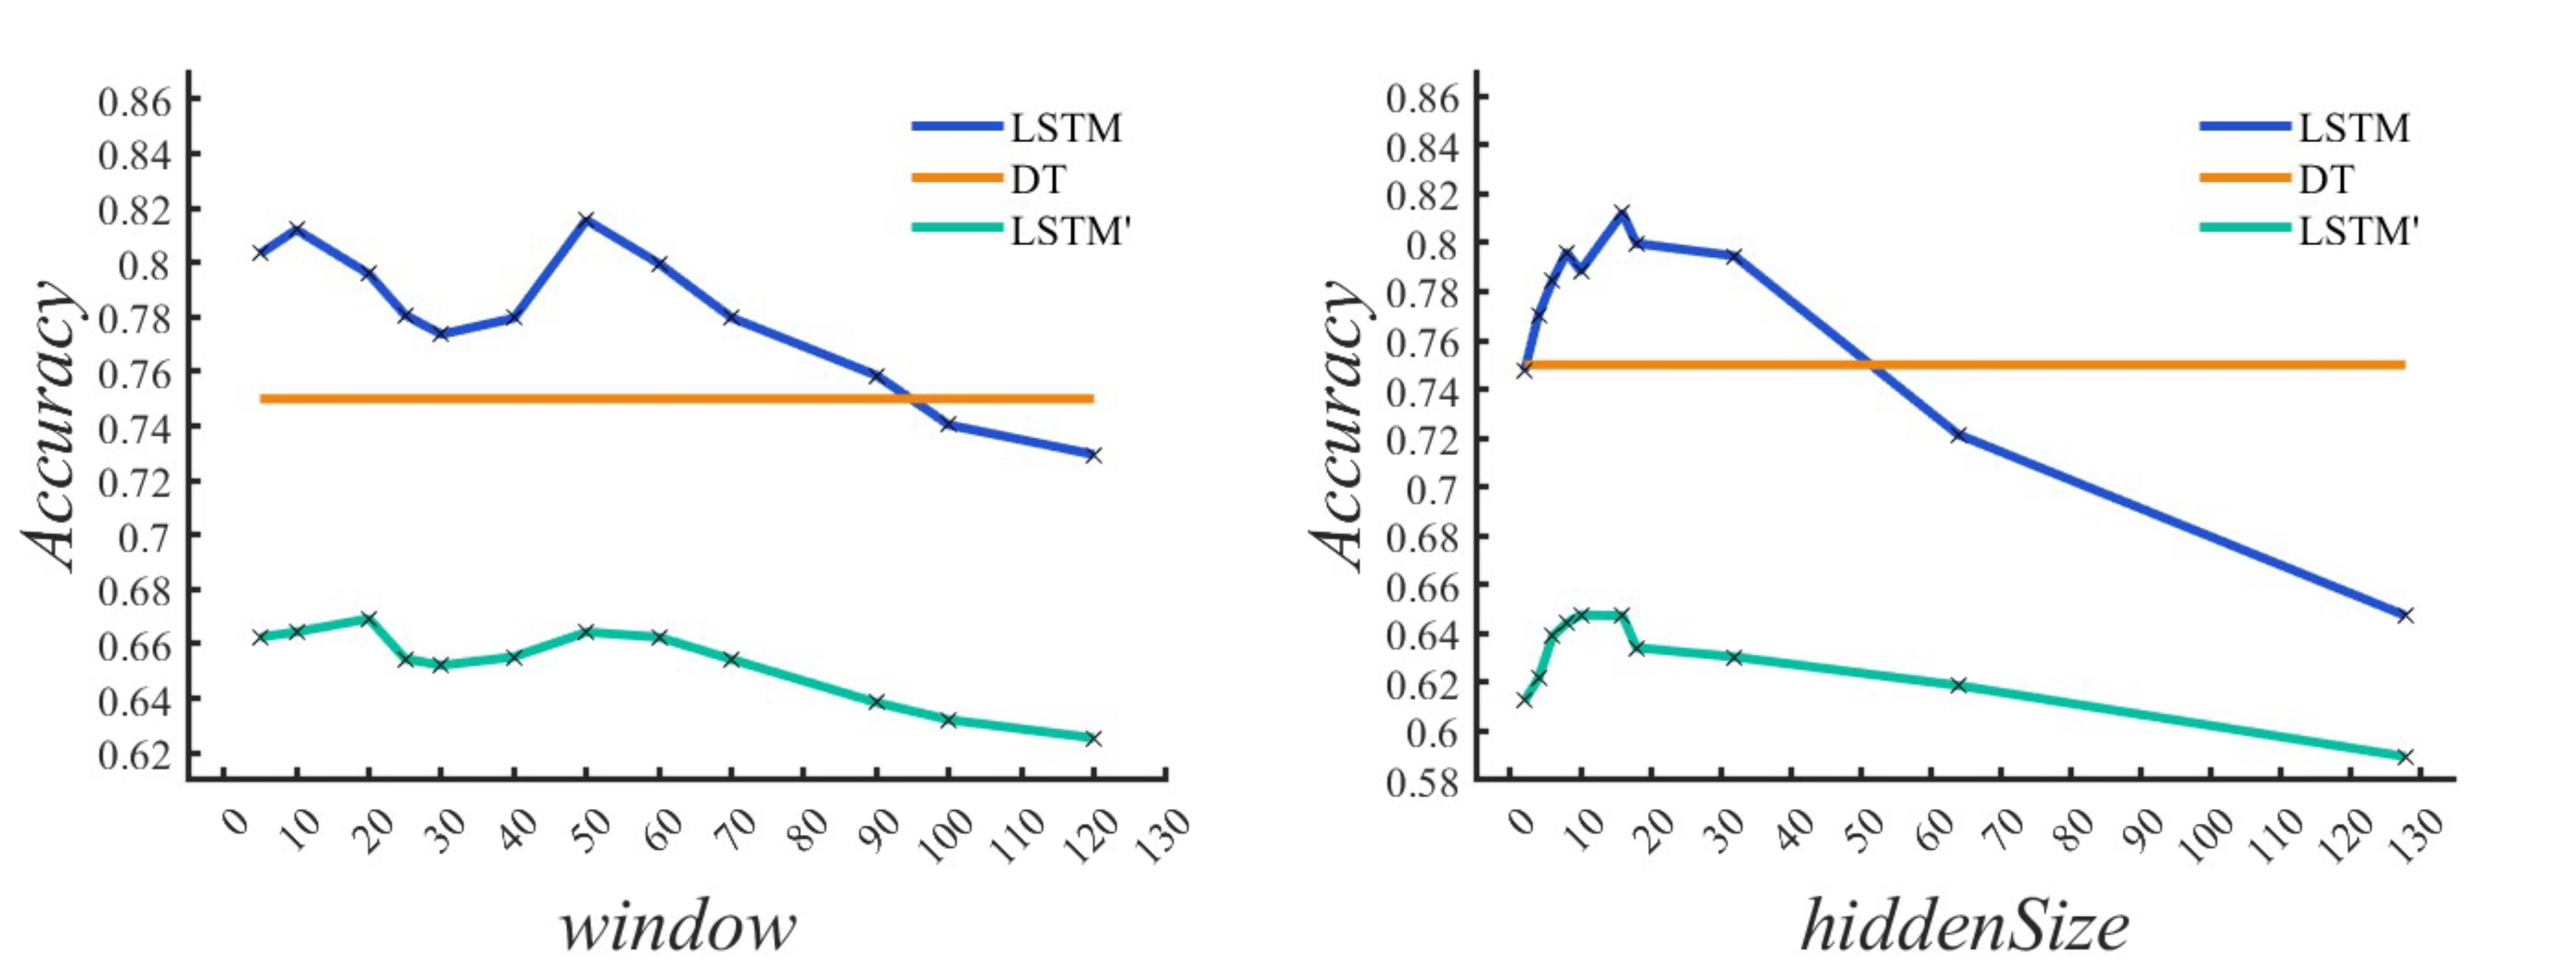
\includegraphics[width=1\linewidth]{figure/lstm3.png}
    \caption{\centering Adjusted LSTM Experiment\\
    \vspace{2pt}
    (LSTM: use main indicators as input, LSTM': remove main indicators)}
    \label{fig:lstm3}
\end{figure}
The results of some of our experiments are shown in Figure \ref{fig:lstm3}, where the best model achieves an accuracy of \textbf{0.81} and the model without using main indicators as input perform poorly. This indicates that we chose the right indicators in the decision tree part and the success of the adjustment we've made to the lstm model as described above.

\subsubsection{Discussion}
\textbf{Window Size: }
    We further discussed the window size discussed in question 2. In the model built in question 3, window size has an impact on model performance, which indicates that the model built in question 3 makes better use of the LSTM's advantage, which is utilizing long and short-term memory. It also suggested that for the LSTM model, the raw data should not be processed too much, which is more favorable for the model to obtain information.

\subsubsection{Suggestions}
Based on the statistics we've got, Athletes need to focus on the influences of the serve, the game situation, the winner of the previous game, etc., during the match. We also experimented with the influence of different situations through the Decision Tree. For example, we tested whether a score of 40 plays a more important role than a score of 30. The results show that there is very little difference in their impact and it depends on the players' own characteristics. Different players react differently to the same situation. \par

We recommend focusing on these main factors and designing tactics with his characteristics. Maximize the duration of his side's advantage and minimize fluctuations in the game that are not in his favor. \par


\subsection{question 4: Model Expansion and Generalization}
\subsubsection{Model Test Results}
\begin{figure}[bt!]
    \centering
    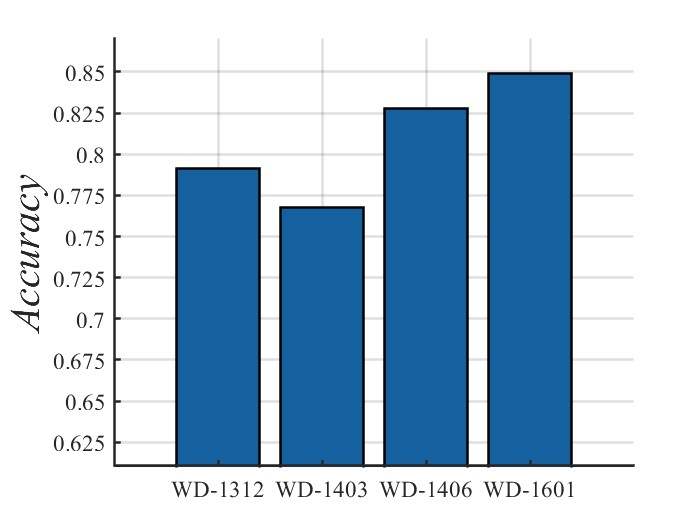
\includegraphics[width=0.5\linewidth]{figure/lstm4.png}
    \caption{\centering Prediction in some matches}
    \label{fig:lstm4}
\end{figure}
As stated before our model training has been based on all the data provided by the problem, so all our previous prediction results are for all matches. In Figure \ref{fig:lstm4} we provide a set of partial results from the test set.\par
As shown in the graph, the prediction accuracy fluctuates from match to match, and we believe that this is due to fluctuations caused by differences in players, etc. from match to match. This again illustrates the importance of introducing player-targeted analysis. \par


\subsubsection{Model Expansion}
When predicting the outcome of a tennis match, it is important to realize that the outcome of the match is not only determined by factors such as the situation on the court, player errors, etc. but is also affected by a combination of factors. We believe that to build a comprehensive and reliable predictive model, a range of key variables must be considered. These variables are summarized as follows:
\begin{itemize}
    \item \textbf{Age of Athlete}\\
    It can be seen from the reference \cite{ref3} that as the age increases, the speed and explosive power of tennis players will reach their peak. It can also be seen from the diagrams excerpted from the Figure \ref{fig:ECAG} that athletes' physical abilities will gradually reach their peak as they grow older during adolescence. As we age, our physical capabilities also decline. When predictive modeling of athlete physical condition, relying solely on observed running distance during a game to predict physical condition would be a simplistic approach. Instead, a more comprehensive and objective assessment of an athlete's physical condition can be achieved by quantifying physical capabilities relative to their age.
    \begin{figure}[b!]
        \centering
        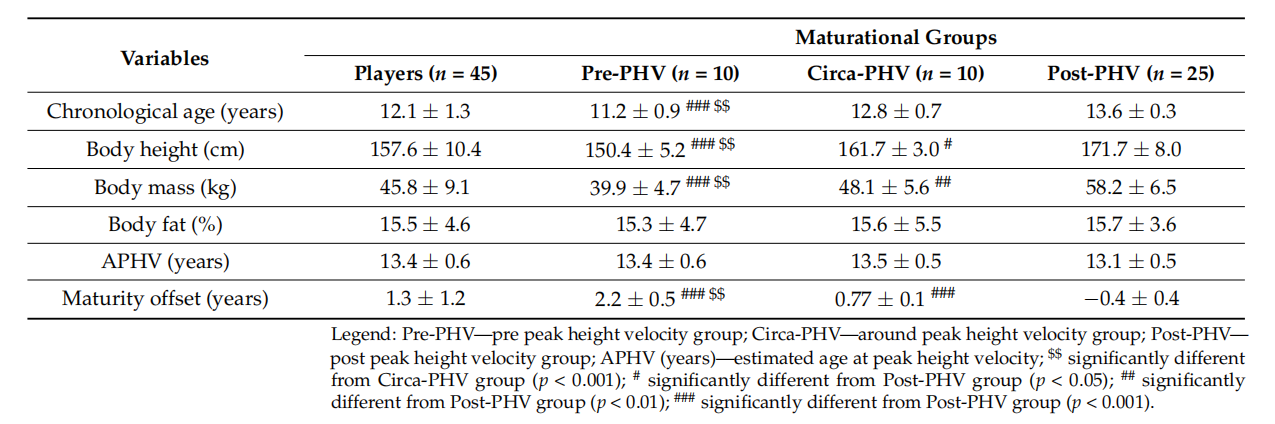
\includegraphics[width=0.75\linewidth]{figure/d021c08d7368ca795e638142b768207.png}
        \caption{\centering Extract Charts and Graphs}
        \label{fig:ECAG}
    \end{figure}

    
    \item  \textbf{Athlete Injuries and Illnesses}\\
    Based on the referenced document \cite{ref4}, it is clear that an athlete's injury status can significantly impact their performance. Injuries can profoundly affect technical aspects such as flexibility, speed, and strength. For instance, an injury to the lower extremities could result in reduced acceleration or impaired agility during directional changes. \\
    The repercussions of injuries are not limited to physiological aspects; they can also exert considerable psychological stress on athletes. Players dealing with injuries often face increased mental pressure during competitions, which can considerably impede their performance. \\
    Therefore, the incorporation of injury status into predictive models is essential. This includes current and past injuries and the probability of re-injury or aggravation based on the athlete's medical history and the nature and frequency of play. By factoring in this information, predictive models can offer a more accurate depiction of a player's potential performance by adjusting for the limitations and psychological burdens that injuries may impose.
    \item \textbf{Player Tactics}\\
    In the realm of tennis, a competitive sport wherein proficiency in technical skills and strategic confrontations over the net with rackets are paramount, the efficacy of tactical acumen cannot be overstressed. Particularly in tournaments of the highest echelon, the deployment of nuanced tactical endeavors is often the crucible within which the fates of matches are forged. Proactive and insightful analyses of adversaries' technical proclivities, both in pre-match preparations and amidst the fray, coupled with the formulation and adroit execution of bespoke tactical blueprints, have frequently tilted the scales in favor of the ostensibly underdog contestant, yielding substantial dividends from ostensibly marginal inputs.\\
    Such assertions are substantiated by empirical inquiries, notably that of Jie Zhang \cite{ref5}, whose scholarly scrutiny into Novak Djokovic's application of techniques and tactics throughout the season of 2021 stands as a testament to the aforementioned. By harnessing the composite research methodologies of entropy weighting and grey relational analysis, Zhang's work methodically appraised Djokovic's exhibition of tactical prowess across a spectrum of competitive engagements, and profoundly elucidated the critical influence such strategic maneuvers exert upon the dynamics and eventualities of high-caliber tennis contests.In reference \cite{ref6}, Maoying Lin also mentioned the technical and tactical characteristics of Alcarás
\end{itemize}

In addition to the above three determinants that profoundly affect the performance of tennis players - technical skills, tactical foresight and tactical adaptability in the game, there are also many factors that need to be considered in modeling, such as the psychological stress tolerance of athletes. needs to be taken into account; in this mentally demanding sport, mental resilience and the ability to cope with high-pressure situations often determines the winners and losers. By considering an athlete's psychological soundness, which includes factors such as mental toughness, researchers and practitioners can gain a more complete and precise understanding of game progression and its outcomes.

\subsubsection{Model Generalization}
\begin{itemize}
    \item \textbf{Applicable to Other Tennis Competitions}\\
    In the process of predicting other tennis matches, we believe that this model has good versatility. However, there may also be situations where the forecast results fluctuate greatly. In order to improve the accuracy of the forecast, the following parameters may need to be adjusted.

- \textbf{Competition Rules}\\
    Different tennis competitions will have some differences in competition rules. For example, Grand Slam events usually include the Australian Open, French Open, Wimbledon and US Open. These games differ in some rules. For example, in the men's singles section, Wimbledon and the US Open adopt an extension system, that is, after the game enters the final set, a tiebreak is required to determine the outcome. At the Australian Open and French Open, players must win six consecutive games to win the deciding set. Therefore, we need to adjust parameters according to different rules in terms of the situation on the field;

- \textbf{Arena Venue}\\
   The types of surfaces used in international tennis events are hard courts, clay courts and grass courts. The Australian Open and the US Open use hard courts, with faster ball speeds and higher rebounds; the French Open is the only clay-court Grand Slam event, with slower courts and relatively slower ball speeds; Wimbledon uses grass courts, with fast ball speeds and low rebounds. Each venue type has different characteristics, which affects the player's playing style and game style. Players need to adjust their strategies and techniques according to the playing surface to cope with the challenges posed by different venues. Therefore, the player's performance also needs to be analyzed on the player's previous game data in different venues to enhance the accuracy of the analysis;

- \textbf{Gender}\\
   There are some differences in the physical fitness of male and female tennis players. Men generally have greater muscle mass and strength potential, can generate greater hitting power, and possess greater acceleration and lateral speed. They also have higher oxygen endurance and resistance to fatigue. Female players are relatively more flexible and have better coordination and body control. Therefore, it is necessary to add the impact of gender factors on player performance;
    \\
    \item \textbf{Applicable to Other Competitions}\\
    Due to the differences between tennis and other sports, this model is less effective in predicting other games such as table tennis, badminton, etc. The main reasons are as follows:\\
    \textbf{-Different physical fitness requirements}\\
    Different sports have different requirements for players’ physical fitness such as strength, endurance, speed, flexibility and coordination. For example, table tennis requires extremely fast reaction speed and delicate hand-eye coordination, while badminton emphasizes speed and endurance.\\
    \textbf{- Differences in Sports Rules and Venues}
    \\ The rules between sports are very different, resulting in great differences in the process and format of the competition. The tennis court is larger than badminton and table tennis, so the players' movement trajectories and playing styles are different.\\
    \textbf{- Differences in Training and Strategies}\\
    Training methods, preparation and competition strategies vary greatly in each sport, which also affects the results of the competition.
\end{itemize}

